
\documentclass[ms.tex]{subfiles}
\begin{document}

\section{Mock Samples}
\label{sec:mocks}

\subsection{A Fiducial Mock Sample}
\label{sec:mocks:fiducial}

\begin{itemize}

	\item We use our parametrization of one-zone GCE models described
	in~\S~\ref{sec:onezone} to set up an underlying model from which
	mock samples can be drawn; we then use a fiducial mock sample to describe
	our fitting method in~\S~\ref{sec:fitting} and explore variations
	in, e.g., sample size and precision.

	\item We take an exponential infall history described by
	\begin{equation}
	\dot{M}_\text{in} \propto e^{-t/\tau_\text{in}}
	\end{equation}
	with~$\tau_\text{in} = 2$ Gyr and an initial gas mass of 0.
	The overall normalization of the infall history is irrelevant because
	mass information cancels in one-zone models when you compute abundances.
	We additionally select~$\tau_\star = 15$ Gyr and~$\eta = 10$ with the
	thought that slow star formation and strong outflows would mimic the
	evolution seen in a typical field dwarf galaxy.
	We set the onset of star formation~$\tau = 13.2$ Gyr ago, allowing~$\sim$0.5
	Gyr between the Big Bang and the first stars.
	We evolve this model for 10 Gyr (i.e. the exact ages of the youngest stars
	in the mock sample are~$\tau = 3.2$ Gyr).

	\item {\color{red} YIELDS}

	\item One-zone models produce stellar populations rather than individual
	stars, so if a mock sample of individual stars is to be obtained, we must
	sample from the underlying population.
	Higher mass stellar populations have proportionally more stars than lower
	mass stellar populations, so we take the probability of sampling to be
	proportional to the mass of a population.
	In the interest of mimicing typical observational samples for local group
	dwarfs, we take~$N = 500$ stars with abundance uncertainties of
	$\sigma\afe = \sigma\feh = 0.05$.
	100 of these stars have age information with an uncertainty
	of~$\sigma\logage = 0.1$.

	\item We illustrate this sample in Fig.~\ref{fig:fiducialmock}.
	This sample shows a ``knee'' in the~\afe-\feh~diagram near~\feh~$\sim$-2.3
	and an equilibrium abundance near~\feh~$\sim$-0.3, but due to the
	declining nature of the SFH, most of the stars form in
	the~\feh~$\sim$-1 and~\afe~$\sim$+0.2 region of chemical space.

\end{itemize}

\subsection{Recovered Parameters of the Fiducial Mock}
\label{sec:mocks:fiducial_fit}

\begin{figure*}
\centering
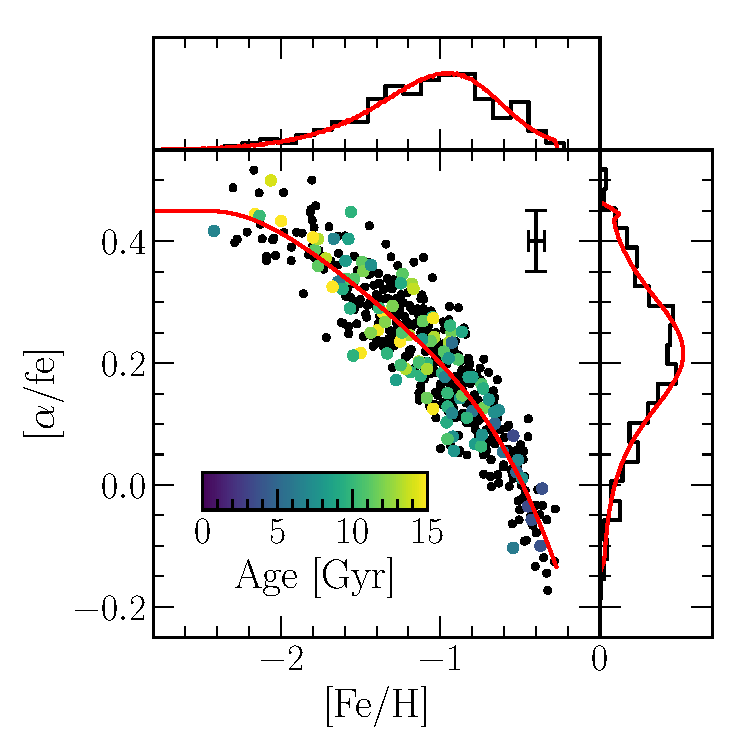
\includegraphics[scale = 0.5]{fiducial_mock_afe_feh.pdf}
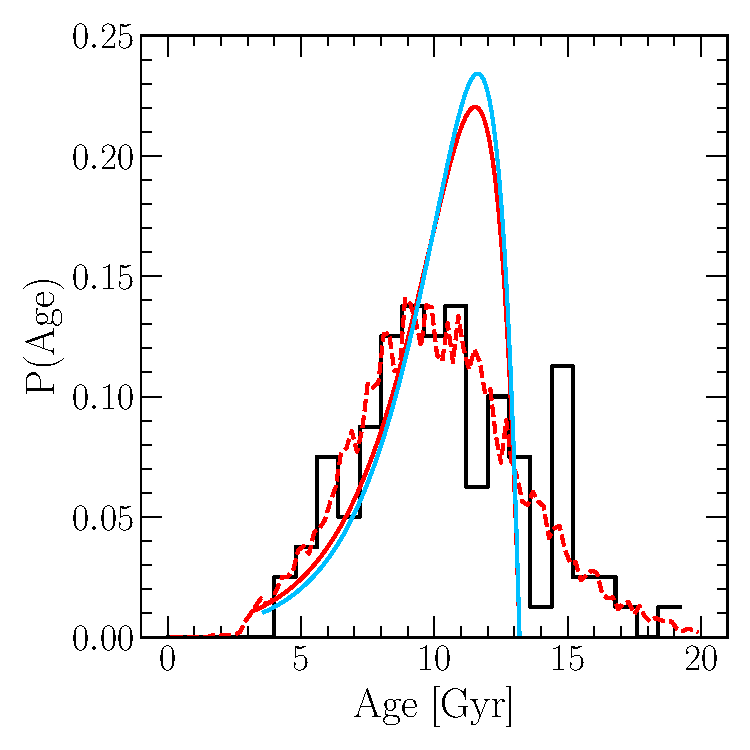
\includegraphics[scale = 0.42]{fiducial_mock_agedist.pdf}
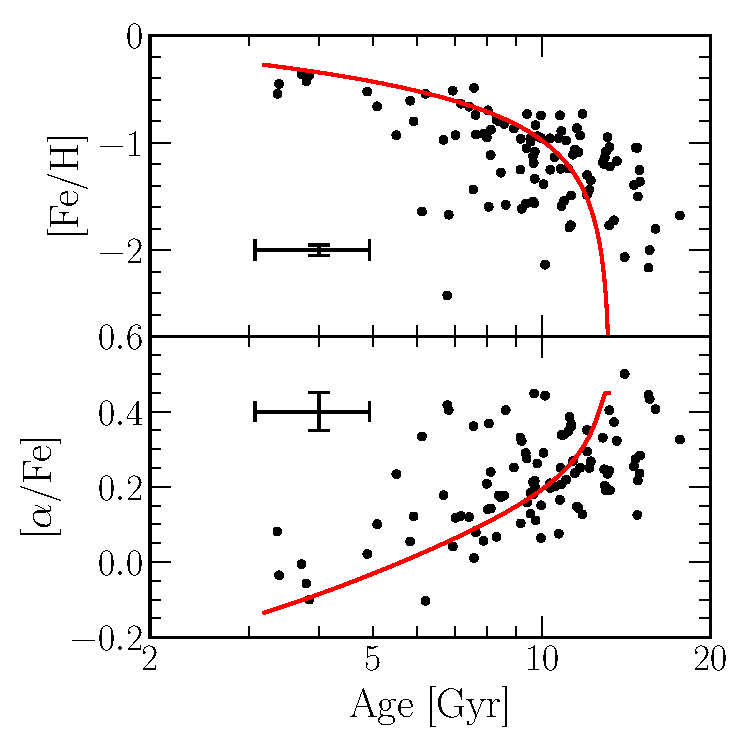
\includegraphics[scale = 0.42]{fiducial_mock_amr.pdf}
\caption{
\textbf{Left}: Our fiducial mock sample in the~\afe-\feh~plane.
There are~$N = 500$ stars with abundance uncertainties
of~$\sigma(\feh) = \sigma(\afe) = 0.05$ as indicated by the errorbar.
$N = 100$ of the stars have age information available with an artificial
uncertainty of~$\sigma(\log_{10}(\text{age})) = 0.1$ as indicated by the
colorbar.
The red line denotes the evolutionary track in the gas-phase from the one-zone
model that generated the mock.
On the top and right, we show the marginalized distributions
in~\afe~and~\feh, with red lines denoting the known distribution.
\textbf{Center}: The mock (black, binned) and known (red) age distributions.
The dashed red line indicates the age distribution that is obtained by sampling
$N = 10^4$ rather than $N = 500$ stars and assuming the same age uncertainty
of~$\sigma(\log_{10}(\text{age})) = 0.1$.
\textbf{Right}: The age-\feh~(top) and age-\afe~(bottom) relation for the mock
sample, with artificial uncertainties denoted by the error bars on each panel.
The red lines denotes the known relations for the gas-phase.
}
\label{fig:fiducialmock}
\end{figure*}

\begin{figure*}
\centering
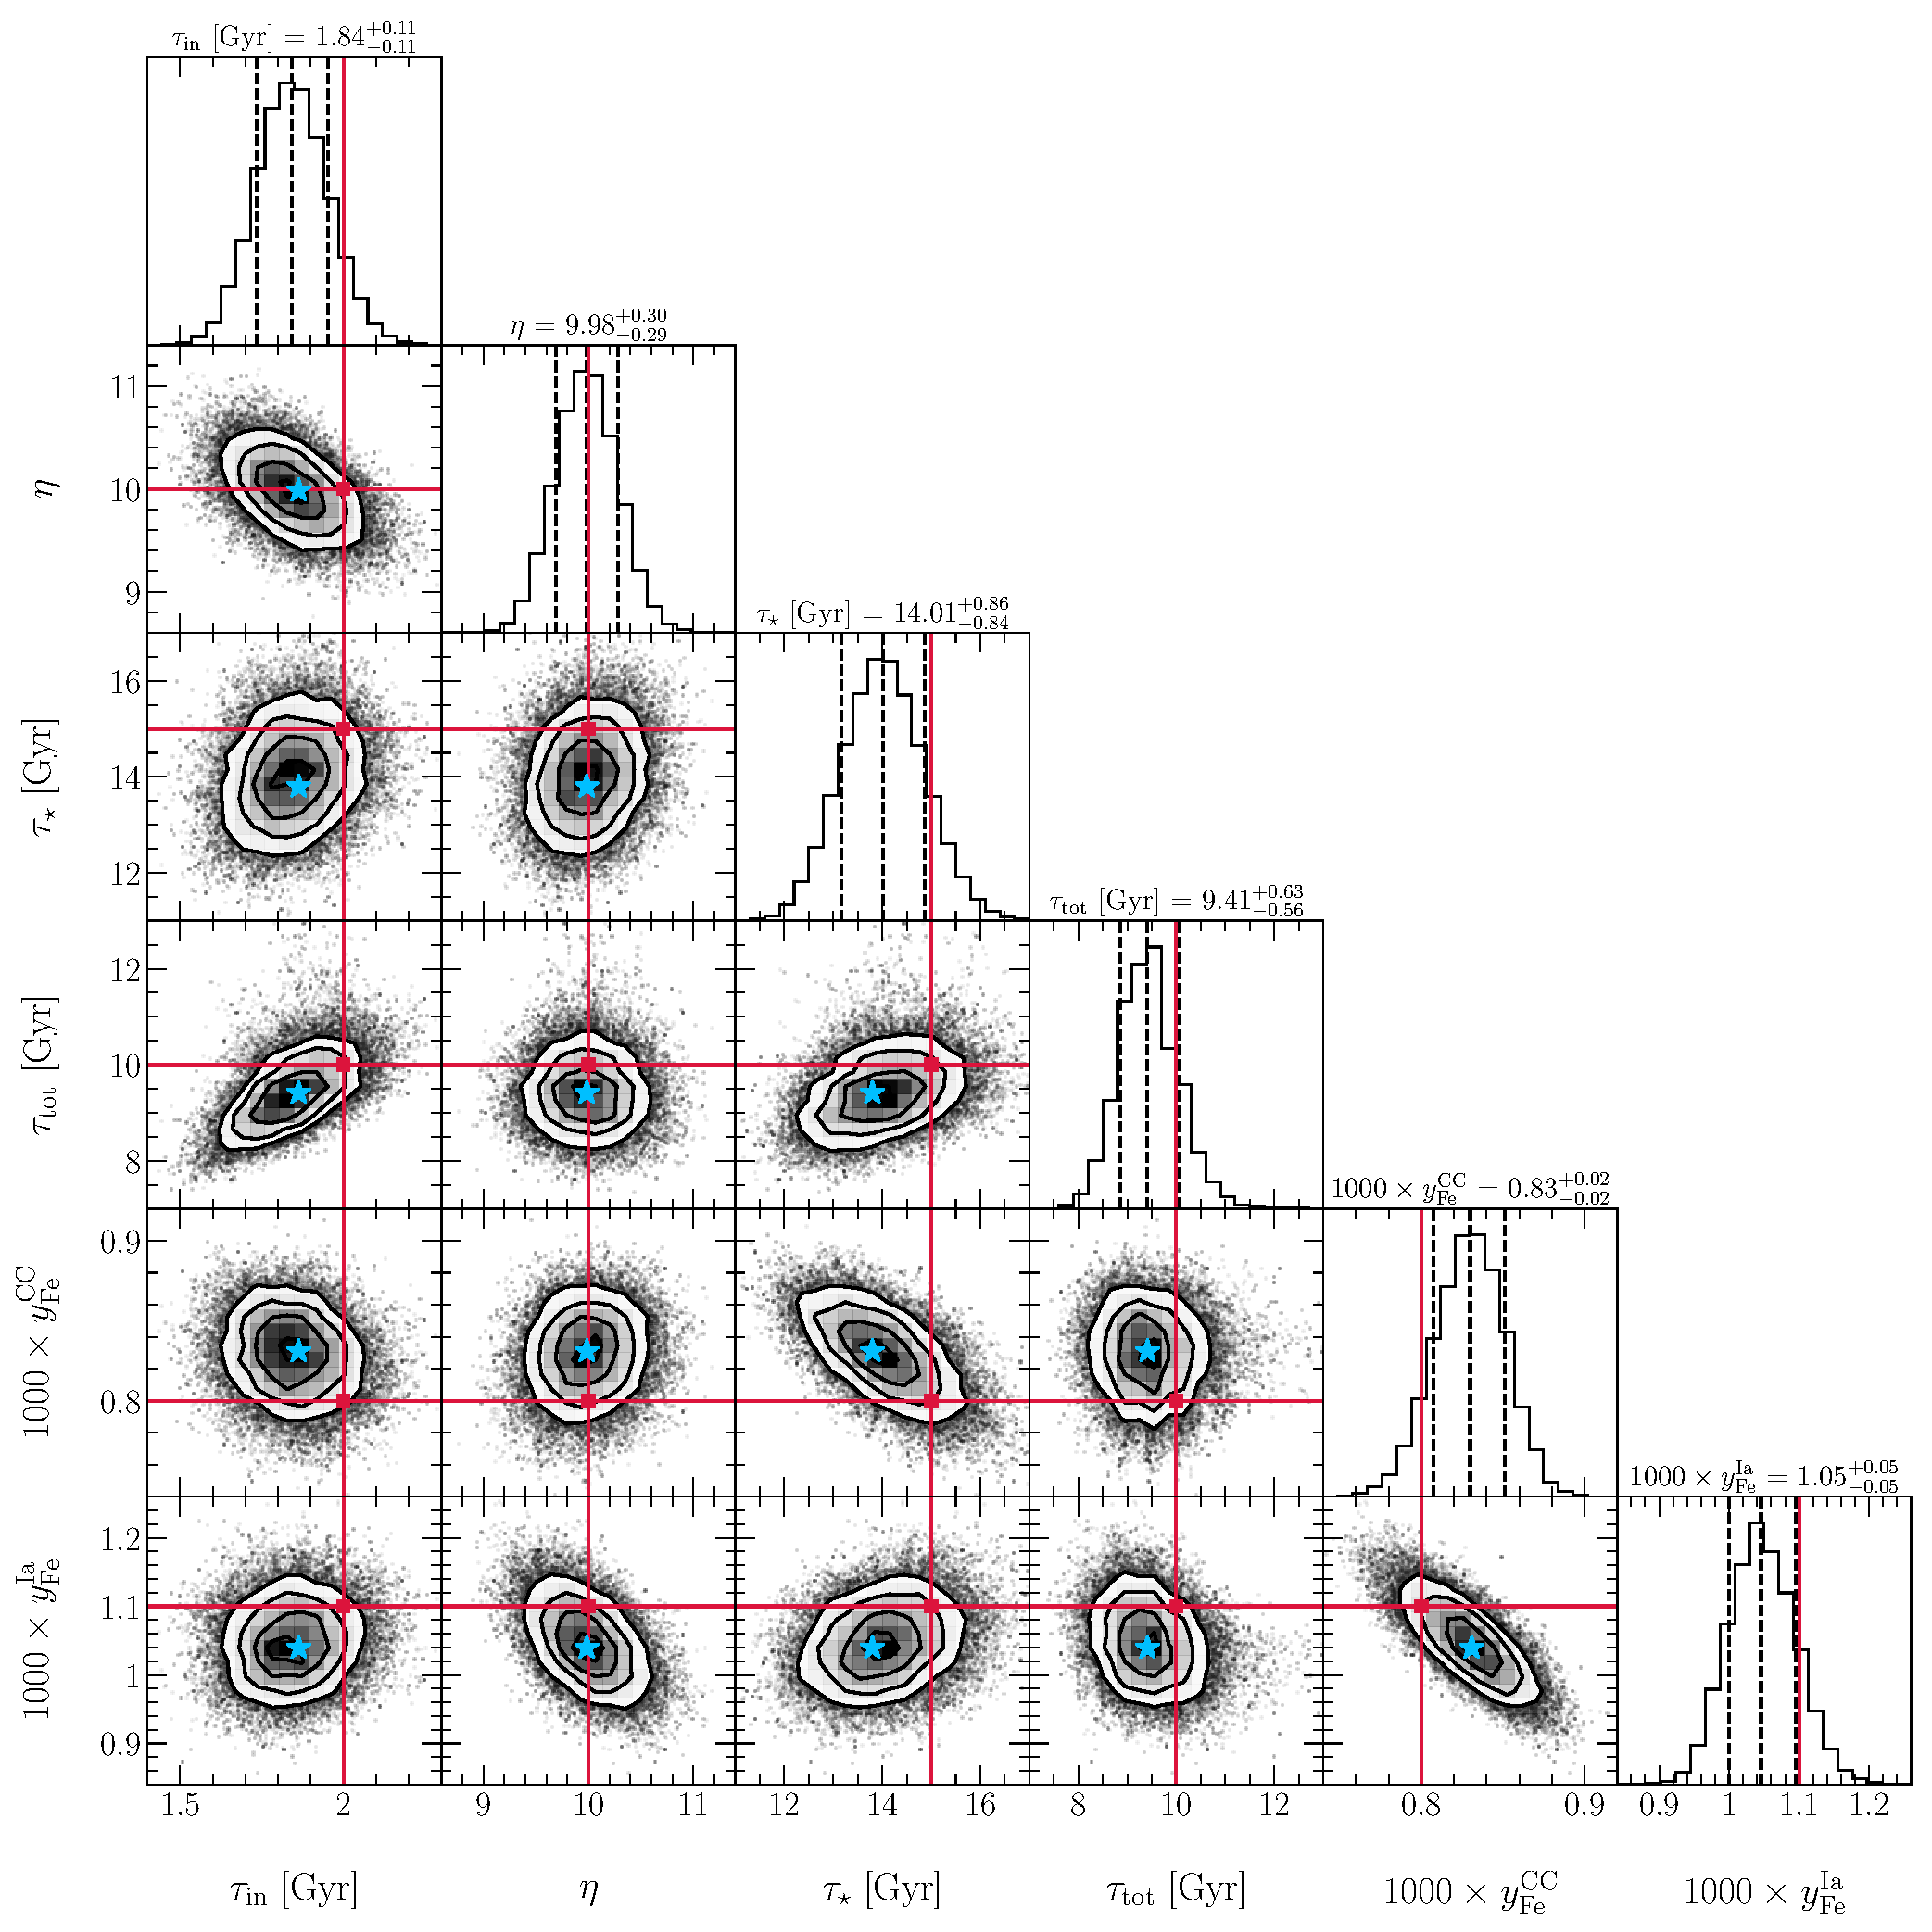
\includegraphics[scale = 0.45]{fiducial_76k8.pdf}
\caption{
The ``corner-plot'' showing the results of applying our fitting method to our
fiducial mock sample (see discussion in~\S\S~\ref{sec:fitting}
and~\ref{sec:mocks:fiducial}).
We show the marginalized likelihood distributions in each parameter along with
their best-fit values and confidence intervals along the diagonal.
Below the diagonal, we show the 2-dimensional cross-sections of the
6-dimensional likelihood function.
Blue stars mark the element of the Markov Chain with the maximum likelihood.
Red ``cross-hairs'' denote the true, known values of the parameters which were
used to generate the mock sample (see the top row of
Table~\ref{tab:recovered_values}).
}
\label{fig:corner_fiducial}
\end{figure*}

\begin{figure*}
\centering
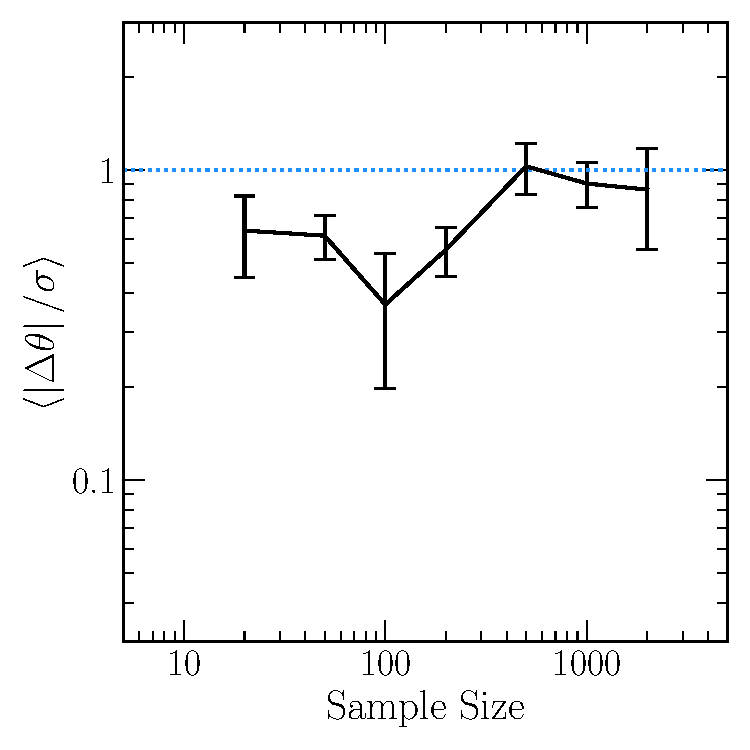
\includegraphics[scale = 0.45]{dp_sigma_samplesize.pdf}
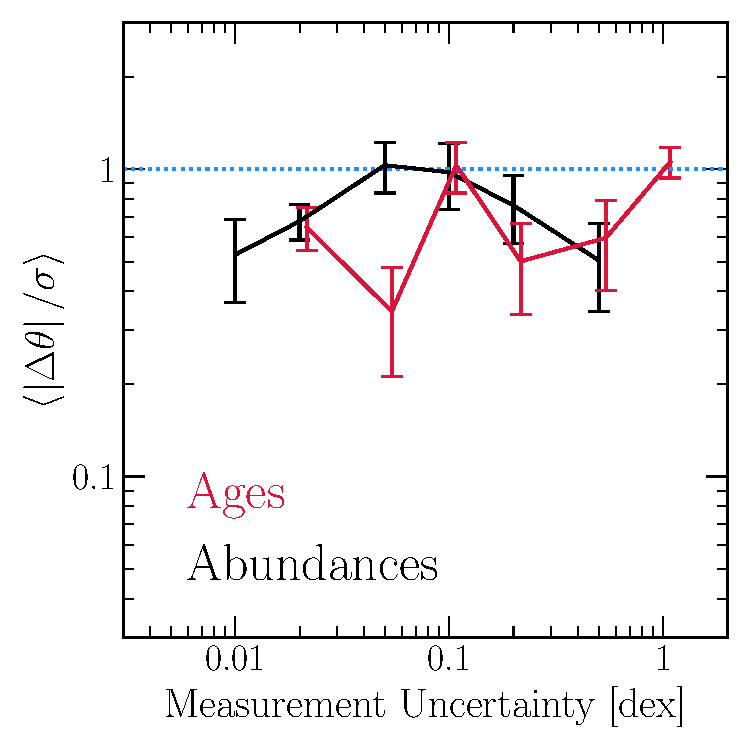
\includegraphics[scale = 0.45]{dp_sigma_precision.pdf}
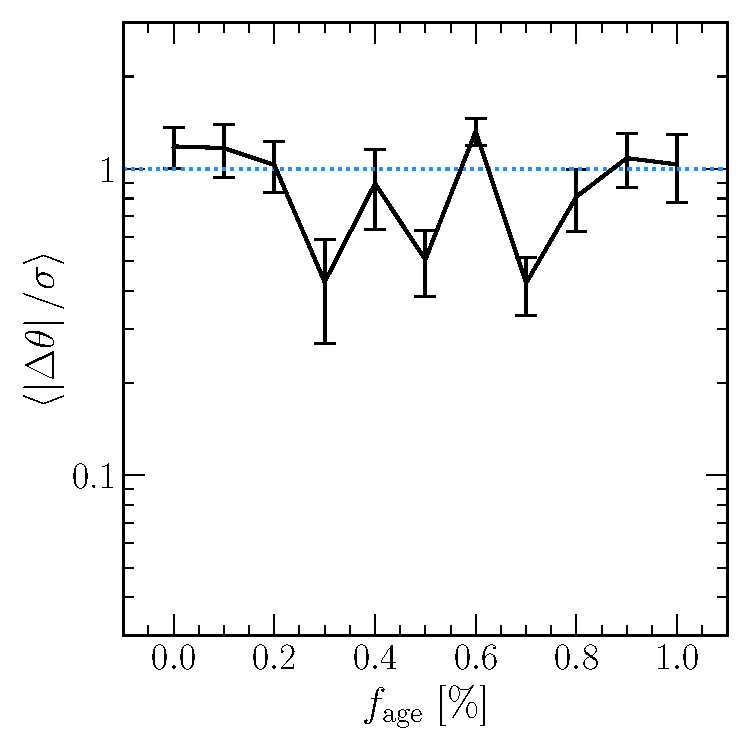
\includegraphics[scale = 0.45]{dp_sigma_agefrac.pdf}
\caption{
The mean deviation between the re-derived mock sample parameters~$\{\theta\} =
\{\tau_\text{in},~\eta,~\tau_\star,~\tau_\text{tot},~\yfecc,~\yfeia\}$ and
their known values from the mock sample in units of the uncertainty on the
best-fit values as a function of the sample size of the mock (left),
measurement precision in abundances~\feh~and~\afe (middle, black),
measurement precision in~$\log_{10}(\text{age})$ (middle, red),
and the fraction of the sample with available age information (right).
Error bars denote the error on the mean deviation in the six parameters.
Blue dotted lines mark~$\langle\Delta\theta/\sigma\rangle = 1$, the
expected value of the mean deviation for a Gaussian random process.
}
\label{fig:dp_sigma}
\end{figure*}

\begin{itemize}

	\item We apply the method outlined in~\S~\ref{sec:fitting} to the
	mock sample detailed in~\S~\ref{sec:mocks:fiducial}.
	Fig.~\ref{fig:corner_fiducial} shows the ``corner-plot'' derived from this
	procedure.
	Along the diagonal, we show the marginalized likelihood distributions in
	each parameter along with their best-fit values and confidence intervals.
	Below the diagonal, we show 2-dimensional cross-sections of the
	6-dimensional likelihood function.
	Blue stars mark the element of the Markov Chain with the highest value
	of~$\ln L$, and red ``cross-hairs'' denote the true, known values of the
	parameters from the mock sample (see the top row of
	Table~\ref{tab:recovered_values}).

	\item Our fitting method is able to accurately recover the known
	evolutionary parameters of the mock sample.
	Although it may appear that there are a high number of~$\gtrsim1\sigma$
	discrepancies, we demonstrate in~\S~\ref{sec:mocks:variations} that the
	differences between the known and best-fit values here are consistent with
	a Gaussian random process associated with measurement uncertainty.

	\item We note a handful of degeneracies in the likelihood distributions of
	the recovered parameters which arise as a consequence of having impact on
	the same observable.

	\begin{itemize}

		\item \textit{The centroid of the MDF.}
		With a fixed alpha element yield of~$\yacc = 0.01$ as we have adopted
		here, the strength of outflows~$\eta$ is set by ensuring the centroid
		of the~\ah~distribution is in agreement with the data.
		This in turn requires a total Fe yield~$\yfecc + \yfeia$ which
		corresponds to the centroid of the~\feh~distribution in the data.
		The total Fe yield, however, can be achieved with different breakdowns
		between CCSN and SN Ia enrichment.
		This gives rise to the inverse relationship between~\yfecc~and~\yfeia~as
		seen in Fig.~\ref{fig:corner_fiducial}.

		\item \textit{The position of the ``knee'' in the evolutionary track.}
		The ``knee'' in the~\afe-\feh~evolutionary track arises with the onset
		of SN Ia enrichment, a nucleosynthetic source of Fe but much smaller
		amounts of alpha elements.
		For fixed yields,~\citet{Weinberg2017} demonstrate that the SFE
		timescale~$\tau_\star$ plays the dominant role in establishing the
		value of~\feh~at which this occurs.
		With low~$\tau_\star$, star formation and consequently enrichment is
		fast, allowing the ISM to achieve a higher~\feh~before the onset of
		SNe Ia.
		However, with the CCSN Fe yield as a free parameter, agreement with the
		data can also be achieved with a higher (lower) value of~\yfecc~and
		slower (faster) star formation.
		This gives rise to the degeneracy between~\yfecc~and~$\tau_\star$ as
		seen in Fig.~\ref{fig:corner_fiducial}.

		\item \textit{The location of the track.}
		Any viable model which reproduces a galaxy's observed abundances in a
		self-consistent manner will predict a track that passes through the
		centroid of the 2-dimensional~\afe-\feh~distribution.
		With other parameters fixed, adjustments to the SN Ia Fe yield move the
		track vertically in the~\afe-\feh~plane (there is horizontal movement
		as well, but the vertical movement is a stronger effect).
		Conversely, the outflow mass-loading factor~$\eta$ is the most dominant
		evolutionary parameter in establishing the equilibrium abundance aside
		from the yields themselves.
		The tug-of-war between the source term of yields and the sink term of
		outflows establishing an equilibrium metallicity was demonstrated as
		early as~\citet{Larson1974} and again more recently
		by~\citet{Weinberg2017}.
		Adjusting~$\eta$ shifts the track horizontally in the~\afe-\feh~plane
		by changing the metal mass retained by the ISM.
		This gives rise to the degeneracy between~\yfeia~and~$\eta$: a change
		in parameter choices which shifts the track down and to the right (or
		up and to the left) may still achieve agreement with the data.

		\item \textit{The shape of the MDF.}
		The~\ah~and~\feh~distributions are affected in a handful of ways by
		these input parameters.
		For sharp infall histories (i.e. low values of~$\tau_\text{in}$), the
		predicted MDF is wider.
		This arises because with a sharp infall history, the gas supply also
		declines sharply with time, and consequently metals are deposited into
		a gas reservoir where the hydrogen and helium lost to star formation
		and outflows is not being replenished (for quantitative justification,
		see discussion in~\citealp{Weinberg2017}).
		These ``gas starved'' galaxies reach higher metallicities than what is
		achieved with a more steadily declining infall history, but a large
		fraction of their stars form early in their evolution when the
		abundances are low.
		As a result, the MDF is wider when~$\tau_\text{in}$ is small.
		\par
		While~$\eta$ establishes the equilibrium abundance in a galaxy for a
		given choice of yields, the SFE timescale describes the spped at which
		the galaxy reaches equilibrium~\citep{Weinberg2017}.\footnote{
			When star formation is fast, Fe is instead limited by the
			timescales associated with the SN Ia DTD, but in the dwarf galaxy
			regime, star formation is generally slow, and it is known to be so
			in this mock sample.
		}
		As a consequence, for a given duration of star formation, a galaxy
		spends less time near its equilibrium abundance when its inefficient at
		forming stars, an effect which increases the weight of low~\feh~stars
		in the MDF.
		Lastly, the duration of star formation~$\tau_\text{tot}$ has the effect
		of cutting off the MDF at some abundance quite literally by stopping
		star formation.
		\par
		Folding all of this together, degeneracies between these parameters
		arise as a consequence of their effects on the MDF.
		Between~$\tau_\text{in}$ and~$\tau_\text{tot}$, a sharp infall history
		can broaden the MDF, but stopping star formation early can cut off the
		MDF, allowing it to retain a peaked shape if the data suggest it.
		Between~$\tau_\text{in}$ and~$\eta$, a sharp infall history increases
		the equilibrium abundance, shifting the centroid of the MDF, but it can
		be lowered by increasing the strength of outflows.
		Between~$\tau_\text{tot}$ and~$\tau_\star$, a fast approach to
		equilibrium can cause the MDF to take on a strong peak, but if star
		formation is stopped early, the frequency of near-equilibrium stars is
		truncated, allowing it to retain a broader shape if the data suggest it.
	\end{itemize}

\subfile{mocksamples.tablebody.tex}

	\item There are additional, weaker degeneracies which can be understood
	by confounding variables.
	For example, the degeneracy between~$\tau_\star$ and~\yfeia~arises because
	both are degenerate with~\yfecc.

	\item We remind the reader that our fits achieve such a precision by
	selecting a scale on which the~$\alpha$ element yield~\yacc~is defined to
	be exactly 0.01 (see discussion in~\S~\ref{sec:onezone:yields}).
	Aside from the infall timescale~$\tau_\text{in}$ and the total duration of
	star formation~$\tau_\text{tot}$, each parameter in this fit is affected by
	the yield-outflow degeneracy.
	We quantify this in detail in Appendix X.

	\item To quantify the quality of the fit, we take the point along the track
	$\script{M}_j$ for each datum~$\script{D}_i$ with the highest statistical
	likelihood~$\ln L(\script{D}_i | \script{M}_j)$ by maximizing the term
	inside both summations in equation (\ref{eq:likelihood}; i.e.,
	$\{\script{M}_j~|~w_j \chi^2 = \max(w_j \chi^2)\}$ where
	$\chi^2 = \exp(-\Delta_{ij}C_i^{-1}\Delta_{ij}^T/2)$ for each
	datum~$\script{D}_i$.
	We then take~$\chi_\text{dof}^2$ to be the sum of the individual
	chi-squared values divided by the total number of individual age and
	abundance measurements minus the six parameters in the fit.
	Although we find that marginalizing over the track~\script{M}~is necessary
	to derive accurate best-fit parameters (see discussion
	in~\S~\ref{sec:fitting}), here we are simply assessing the quality of the
	fit.
	As noted in the middle panel of Fig.~\ref{fig:fiducialmock}, this fit
	achieves~$\chi_\text{dof}^2 = 0.55$, indicating that we have perhaps
	over-fit the mock data.
	This is rather unsurprising, however, given that we have fit the mock data
	with the exact, known parametrization of its evolutionary history in the
	interest of demonstrating its accuracy.

\end{itemize}

\begin{figure*}
\centering
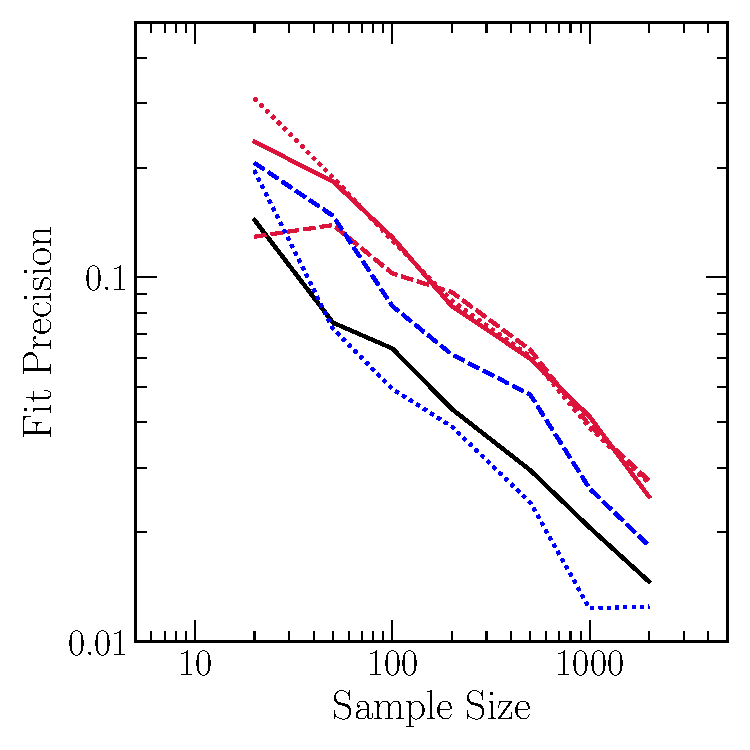
\includegraphics[scale = 0.52]{precision_samplesize.pdf}
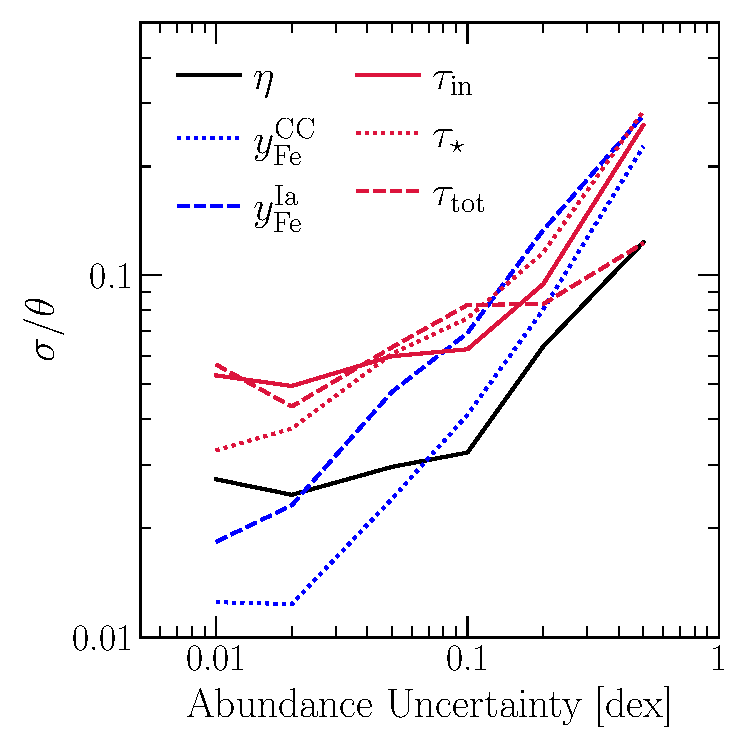
\includegraphics[scale = 0.52]{precision_abundanceuncertainty.pdf}
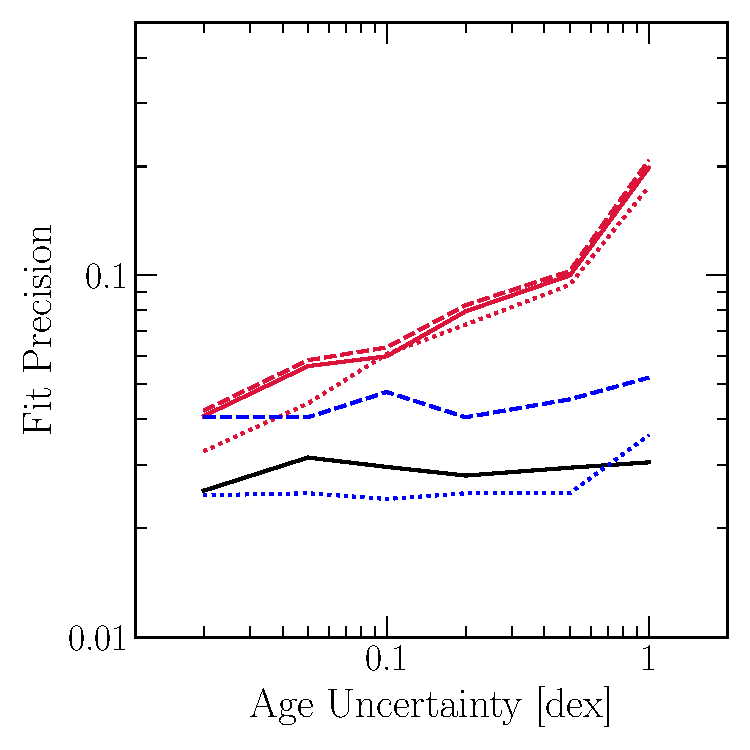
\includegraphics[scale = 0.52]{precision_ageuncertainty.pdf}
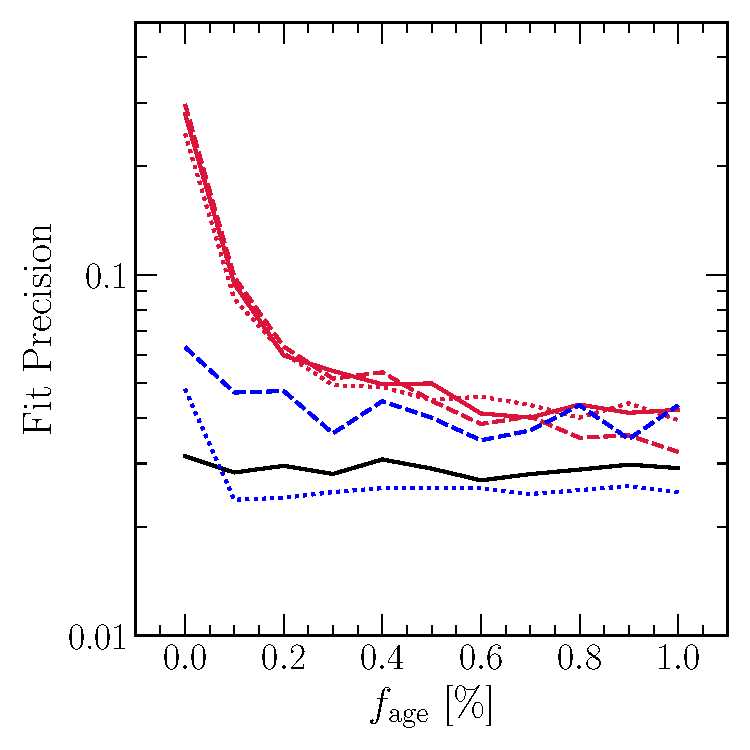
\includegraphics[scale = 0.52]{precision_agefrac.pdf}
\caption{
The precision of our re-derived mock sample parameters~$\{\theta\} =
\{\tau_\text{in},~\eta,~\tau_\star,~\tau_\text{tot},~\yfecc,~\yfeia\}$ as a
function of sample size (top left), measurement uncertainty in~\feh~and~\afe
abundances (top right), measurement uncertainty in~$\log_{10}(\text{age})$
(bottom left), and the fraction of the sample with age measurements (bottom
right).
We plot timescales in red, Fe yields in blue, and the mass-loading factor~$\eta$
in black according to the legend in the upper right panel.
}
\label{fig:precision}
\end{figure*}

\subsection{Variations in Sample Size, Measurement Precision, and the
Availability of Age Information}
\label{sec:mocks:variations}

\begin{itemize}

	\item We now explore variations of our fiducial mock sample with respect
	to sample size, measurement precision, and the availability of age
	information.
	These variations retain all of the evolutionary parameters of the fiducial
	mock, but differ in one of the number of stars in the sample, measurement
	uncertainty in~\feh~and~\afe~abundances, measurement uncertainty
	in~$\log_{10}(\text{age})$, or the fraction of the sample with age
	measurements.
	The left-hand column of Table~\ref{tab:recovered_values} provides a summary
	of the values we take as exploratory cases for each mock variation, with
	the values taken in the fiducial sample highlighted in bold.
	In the remaining columns, we provide the associated values derived for each
	GCE parameter~$\theta$ along with their~$1\sigma$ uncertainties; the true
	values are noted in the top row.
	Our choices in measurement precision are intended to reflect typical values
	achieved by modern spectroscopic surveys where robust age information is
	often available for only a portion of the sample, and may be adopted from
	another source with a precision that is unrelated to the abundance
	uncertainties.
	Our chosen sample sizes are also intended to reflect a typical sample that
	might accurately be described by a one-zone model; with the requirement
	that mixing be efficient, it is likely that only dwarf galaxies meet this
	condition.
	Much more distant than nearby Galactic stars, dwarf galaxies are less
	conducive to the large sample sizes achieved by surveys of the Milky Way
	(e.g. APOGEE and GALAH).
	In larger systems like the Milky Way, processes such as stellar migration
	(refs) and radial gas flows (though perhaps less importantly; refs) have
	been demonstrated to significantly impact the observed abundance
	distributions as well as their evolution.
	This demands a more sophisticated parametrization than a one-zone model
	anyway, prompting a number of authors to explore so-called ``multi-zone''
	GCE models (refs).

	\item Fig.~\ref{fig:dp_sigma} demonstrates the accuracy of our fitting
	method with respect to variations in these details surrounding the data.
	On the y-axis of each panel, we plot the mean deviation between each
	re-derived parameter~$\theta$ (i.e.~$\tau_\text{in}$,~$\eta$,~$\tau_\star$,
	etc.) and its known value from the mock sample normalized according to the
	fit precision on~$\theta$.
	Under all mock variants that we explore, our method recovers the known
	values of the parameters to~$\sim1\sigma$ or slightly better.
	This is exactly as expected when the uncertainties are described by a
	Gaussian random process, for which the most likely deviation from the true
	value is exactly~$1\sigma$, even with infinite data.

	\item This suggests that our method should provide accurate best-fit
	evolutionary parameters even when the sample size is as low
	as~$N \approx 20$, when the measurement uncertainties are as high
	as~$\sigma_\text{[X/Y]} \approx 0.5$ and~$\sigma_\text{log(age)} \approx 1$,
	or even when there is no age information available at all.
	The precision of the fit will indeed suffer in these cases (see Fig.
	\ref{fig:precision} and associated discussion below), but it will remain
	accurate.

	\item We have explored alternate parametrizations of our mock sample's
	evolutionary history and indeed found that our method accurately recovers
	the parameters in each case.
	These ``stress tests'' include a case in which we build in a significant
	starburst, and our method accurately recovers both the timing and the
	strength of the burst.
	We have also explored an infall rate which varies sinusoidally about some
	mean value, mimicing a series of minor starbursts.
	Although idealized and potentially unrealistic, our method accurately
	recovers the amplitude, phase, and frequency in this case as well.

	\item Fig.~\ref{fig:precision} demonstrates how the precision of our
	best-fit parameters is affected by these details of the sample.
	in general, the mass-loading factor~$\eta$ and the Fe yields are
	constrained more precisely than the timescales.
	The primary exception to this rule is when the abundance uncertainties are
	large, in which case the Fe yields are constrained to a similar precision
	as~$\tau_\text{in}$ and~$\tau_\text{star}$, but~$\tau_\text{tot}$ is
	determined more precisely.

	\item All parameters are affected similarly by the size of the sample, with
	the precision scaling approximately as~$\sigma/\theta \propto N^{-0.5}$.
	In other words, a factor of 10 increase in precision on the best-parameters
	$\{\theta\}$ would require a factor of 100 increase in sample size if the
	uncertainties and availability of age information is held fixed.
	Unsurprisingly, the Fe yields are the parameters most sensitive to the
	abundance uncertainties.
	Even with imprecise abundance measurements of~$\sigma_\text{[X/Y]}
	\approx 0.5$, the mass-loading factor~$\eta$ can still be determined to
	$\sim$10\% precision.
	Changes in this parameter shift the observed MDF to higher or lower values,
	but do not affect its overall shape.
	This suggests that even with poorly measured abundances, the centroid of
	the MDF is still robustly determined, allowing a precise measurement of the
	strength of outflows, a quantity which in principle should contain
	information on the depth of the galaxy's gravity well.

	\item With both the availability of age information and the uncertainties
	thereof, only the best-fit precision of timescale parameters are affected.
	Even with order of magnitude uncertainties on stellar ages, however, the
	evolutionary timescales of our mock samples are recovered to~$\sim$20\%
	precision.
	Interestingly, age information affects the precision of best-fit timescales
	only up to~$f_\text{age} \approx 30\%$.
	Above this value, there is only marginal gain in the precision of inferred
	timescales, suggesting that there is a point beyond which additional age
	measurements do not add any new information to the fit.

	\item These results suggest that authors seeking to determine best-fit
	evolutionary parameters for dwarf galaxies using their chemical abundances
	should focus their efforts on sample size and precise abundance
	measurements over age information.
	Thankfully, abundances are considerably easier than stellar ages to measure
	precisely.
	We caution that the level of accuracy and precision quantified here in
	these mock samples is contingent on the galaxy in question being accurately
	described by a one-zone model of chemical evolution.
	Furthermore, the model must be parametrized in such a manner that
	accurately describes the galaxy's evolutionary history.
	For example, if~$\tau_\star$ or~$\eta$ are assumed to be constant while
	they in reality were not, or if an exponential infall history is adopted
	when this is a poor description of the galaxy's evolutionary history, then
	the accuracy and precision of the fit will suffer, as in any statistical
	parameter optimization.
	Standard quality-of-fit diagnostics such as chi-squared per degree of
	freedom are a useful litmus test for such cases.

\end{itemize}

\end{document}

